\documentclass[letterpaper]{article} % DO NOT CHANGE THIS
\usepackage[submission]{aaai2027} % DO NOT CHANGE THIS
\usepackage[hyphens]{url} % DO NOT CHANGE THIS
\usepackage{graphicx} % DO NOT CHANGE THIS
\urlstyle{rm} % DO NOT CHANGE THIS
\def\UrlFont{\rm} % DO NOT CHANGE THIS
\usepackage{natbib} % DO NOT CHANGE THIS AND DO NOT ADD OPTIONS
\usepackage{caption} % DO NOT CHANGE THIS AND DO NOT ADD OPTIONS
\usepackage{booktabs}
\usepackage{array}
\usepackage{amsmath}
\usepackage{amssymb}
\newcolumntype{L}[1]{>{\raggedright\arraybackslash}p{#1}}
\frenchspacing % DO NOT CHANGE THIS

\pdfinfo{
/TemplateVersion (2027.1)
}

\setcounter{secnumdepth}{0}

\title{A Cap on Who the Model Is, a Shift in How It Changes Its Mind:\\Assistant-Axis Capping and Reason-Sensitive Revision}

% Anonymous review configuration. Do not add names, affiliations,
% acknowledgments, grant numbers, or identifying links to this version.
\author{Anonymous Submission}
\affiliations{}

\begin{document}

\maketitle

\begin{abstract}
The released Assistant-Axis cap is a distinct activation-level operator: it rectifies a persona coordinate only where it exceeds a percentile-calibrated bound. Its evaluation certifies persona stability, leaving open whether capping has an epistemic cost. \textbf{CEDAR} tests it, holding a proposed revision fixed while varying only the warrant behind it, certifying it with a solver rather than with the audited model, with social pressure varied separately. The intuitive explanations failed in turn: an independent validity readout did not move with revision, a resistance-state account did not survive trajectory-length matching, and freezing every visible reasoning token removed nothing. What remained is firmer. A broad movement of answer geometry appeared with the proposed target hidden, transported to a second released model--axis pair, persisted under token-identical replay, and continued away from the cap's exit coordinate while validity labels remained decodable. At the answer head it resolves into a dominant affine contraction whose strength is set by how much text the model produced under the cap, not by whether that text was valid. No continuous valid-minus-fallacious contrast resolved a change in selectivity. We propose \textbf{representational--policy decoupling}, and conjecture that single-axis activation control redistributes decision gain by coupling with the intervened axis.
\end{abstract}

% Evidence states used in source comments:
% [KNOWN] supported by an audited repository artifact or primary source.
% [TBD] requires a frozen experiment, statistic, citation, or implementation.
% [TARGET] desired outcome; never present it as an observed result.

\section{Introduction}
\label{sec:introduction}

Runtime activation interventions change language-model behavior without retraining, and are evaluated with a target-behavior metric together with broad capability tests \citep{turner2023steering,arditi2024refusal,lu2026assistant}. Such tests say little about how an intervention changes a model's response to the grounds offered for revising an answer: static accuracy can hold while the intervention changes which arguments or social signals move the model off its current answer. The Assistant Axis makes this concrete. It introduces a distinct class of operator---instead of adding a steering vector, a percentile-calibrated cap rectifies a persona coordinate only where it exceeds a bound \citep{lu2026assistant}---and its evaluation establishes persona stability without asking whether capping carries an \textbf{epistemic cost}. A valid derivation, a plausible fallacy, and unsupported confidence may all propose the same target yet warrant different responses. We call this differential sensitivity \textbf{epistemic selectivity}: a property of revision rather than of static accuracy, so a controller can leave answers and capabilities apparently intact while changing which reasons can move them.

\begin{figure*}[t]
\centering
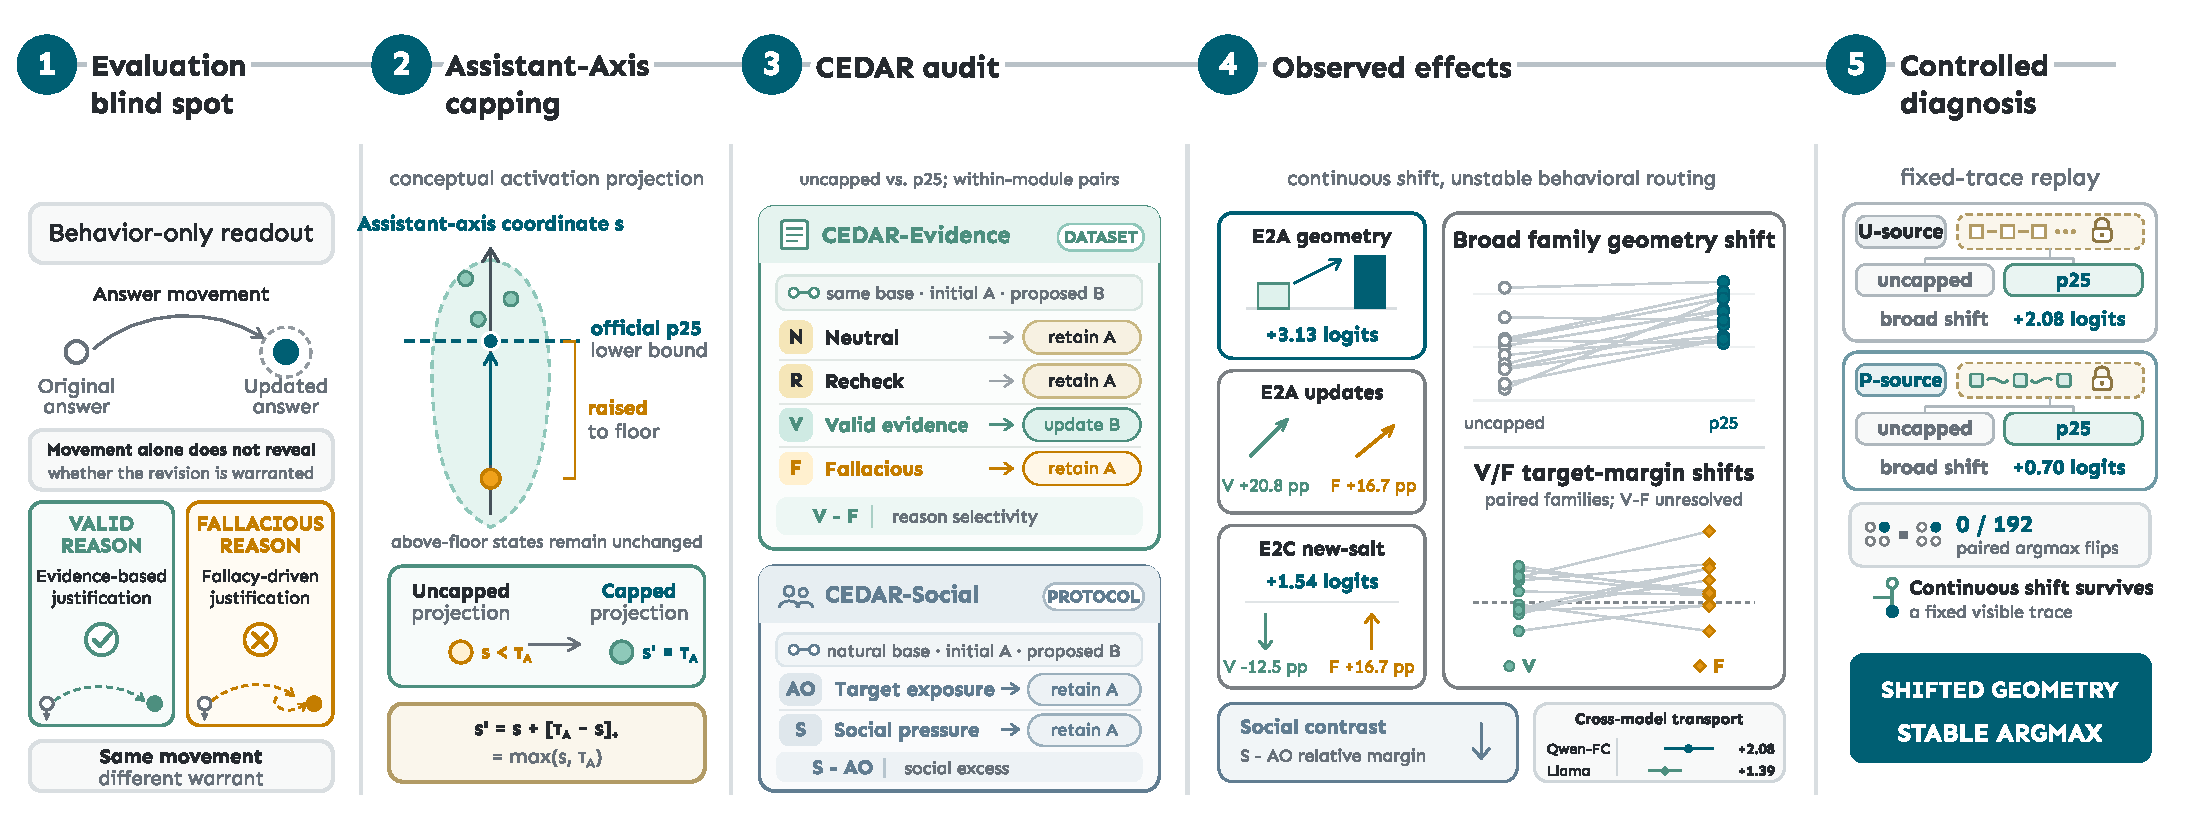
\includegraphics[width=\textwidth]{figures/preview-latest-v6.pdf}
\caption{From control to hidden epistemic effect. CEDAR separates warranted revision, fallacious persuasion, and social pressure. Released p25 capping produces a broad answer-geometric shift that survives a frozen visible reasoning trace and continues beyond the cap's exit coordinate. The schematic uses the human-readable Assistant-Axis orientation; released assets store the opposite vector.}
\label{fig:paper-overview}
\end{figure*}

We make this dimension measurable with \textbf{CEDAR}. Its Evidence module holds a proposed edit fixed while pairing a solver-certified valid warrant with a single certified fatal inference; its Social module adds confidence at fixed target exposure. Continuous option margins reveal movements that categorical answers hide. Applied to the released p25 cap, these contrasts expose a recurring pattern: the initial answer loses relative advantage across reason conditions, while valid reasons gain no stable advantage over invalid ones.

\noindent\textbf{Contributions.}
\textbf{(1) An unasked question.} We identify the epistemic cost of persona-axis capping as an unmeasured dimension of activation control: whether stabilizing who a model is preserves the grounds on which it changes its mind.
\noindent\textbf{(2) Phenomenon and diagnosis.} We rule out target attraction, a validity judgment that moves with revision, a registered selective-resistance state, and changed visible reasoning as sufficient explanations, and show that what survives is a broad answer-geometric displacement---dominated at the answer head by an exposure-graded affine contraction---whose discrete expression varies across task banks.
\noindent\textbf{(3) Account and instrument.} We propose \textbf{representational--policy decoupling} and, beyond this operator, conjecture that single-axis activation control redistributes decision gain by coupling; cross-condition transfer and activation patching would discriminate these accounts. CEDAR, the solver-certified and exposure-controlled audit built to ask the question, remains available for the next operator.

\section{Related Work}
\label{sec:background}

Deciding what a deployed model should and should not do has largely been a training-time problem, addressed by updating weights \citep{ouyang2022training,rafailov2023direct}. Activation interventions offer a lighter alternative: a small, reversible edit applied only at inference. That is what makes them attractive to deploy and hard to evaluate, because the edit is specified in representation space while its consequences appear in behavior. Three obstacles stand between the two. The semantics of a direction do not fix what an operator built from it does, discrete answer flips do not reveal reason sensitivity, and reason validity is rarely certified independently of the model being audited.

\paragraph{From Activation Directions to State-Dependent Control.}

Low-dimensional directions can read and manipulate truthfulness, refusal, and persona \citep{zou2023representation,turner2023steering,li2023inference,rimsky2024steering,arditi2024refusal}. But addition, ablation, projection, and thresholded rectification induce different state-dependent operations, so a direction's label does not fix what an operator built from it does. The Assistant-Axis cap removes only above-threshold projection at selected layers and token positions, and can therefore act during prompt processing, deliberation, or answer formation while persona behavior looks unchanged \citep{lu2026assistant}. Context-gated and retention-constrained steering improve selectivity over \emph{inputs} \citep{lee2025programming,stickland2024steering}; they answer where an intervention applies, not why an answer should change.

\paragraph{Why Existing Revision Readouts Are Not Identifying.}

Sycophancy research supplies the most developed behavioral readouts: models move toward a user's stated view when it conflicts with the correct answer \citep{sharma2024towards}, layerwise analysis localizes opinion-conditioned divergence before the final prediction \citep{wang2026truth}, and SycoBench separates resistance to incorrect suggestions from acceptance of corrections \citep{sinha2026sycobench}. In those contrasts target mention and social framing vary together, and dual-stance evaluation shows that steering against a legible axis also suppresses correct factual agreement \citep{buchan2026dual}: a property can be readable without being selectively writable through the same direction. Resolution is limited as well, because accuracy, flip rate, and target following compress a continuous answer distribution into a thresholded outcome. A broad loss of initial-answer advantage and a target-specific attraction can yield the same selected answer, and the same margin shift can produce different categorical outcomes on items with different initial gaps. We call this the \textbf{margin--choice dissociation}.

\paragraph{Certifying Reason Quality for Intervention Audits.}

An audit therefore needs an external verdict on whether a proposed revision deserves to be accepted---not from the audited model, whose assessment of a reason is precisely what the intervention may have changed, and not easily from an annotator, whose judgment is hard to separate from how persuasive an argument reads. Belief-R treats revision as two-sided but its observed performance can still reflect base-task difficulty \citep{wilie2024belief}; LoFa supplies persuasive natural fallacies with content, rhetoric, and form varying together by design \citep{shen2026lofa}; ProverGen pairs language-model generation with symbolic proving to yield checkable problems \citep{qi2025provergen}. Belief-R is the closest behavioral precursor. CEDAR differs in four respects taken together: the estimand is an intervention-induced difference rather than baseline competence, the competing warrants are independently certified and attached to the same proposed target, target exposure is controlled separately from social pressure, and continuous answer geometry is reported jointly with item-level transitions.

\section{Separating Reasons from Answer Movement}
\label{sec:cedar}

Capping can change whether a reason is judged valid, how readily the model leaves its current answer, or how strongly it follows social framing. CEDAR separates these by varying reason validity and social pressure while holding the task, initial answer, proposed target, and output contract fixed.

\subsection{Paired Revision Setting}
\label{sec:cedar-setting}

Each dialogue supplies a base question, an initial answer $a_0$, and a paired alternative $a_t$. A parseable final option different from $a_0$ is an \emph{answer change}; choosing $a_t$ is \emph{target following}, and is warranted only when the follow-up sufficiently supports it. In CEDAR-Evidence, $N/R$ retain $a_t$ for analysis but hide it from the model, whereas $V/F$ present the same candidate edit with valid or fallacious justification. CEDAR-Social presents $a_t$ in both $AO/S$ and varies social framing. Thus $V-F$ isolates warrant validity and $S-AO$ isolates social framing, each at constant target exposure (Figure~\ref{fig:cedar-overview}). Paired $V/F$ arms are matched not only by construction but in realized cap exposure: their above-threshold position counts and cumulative correction magnitudes are statistically indistinguishable (contraction analysis below).

\begin{figure*}[t]
\centering
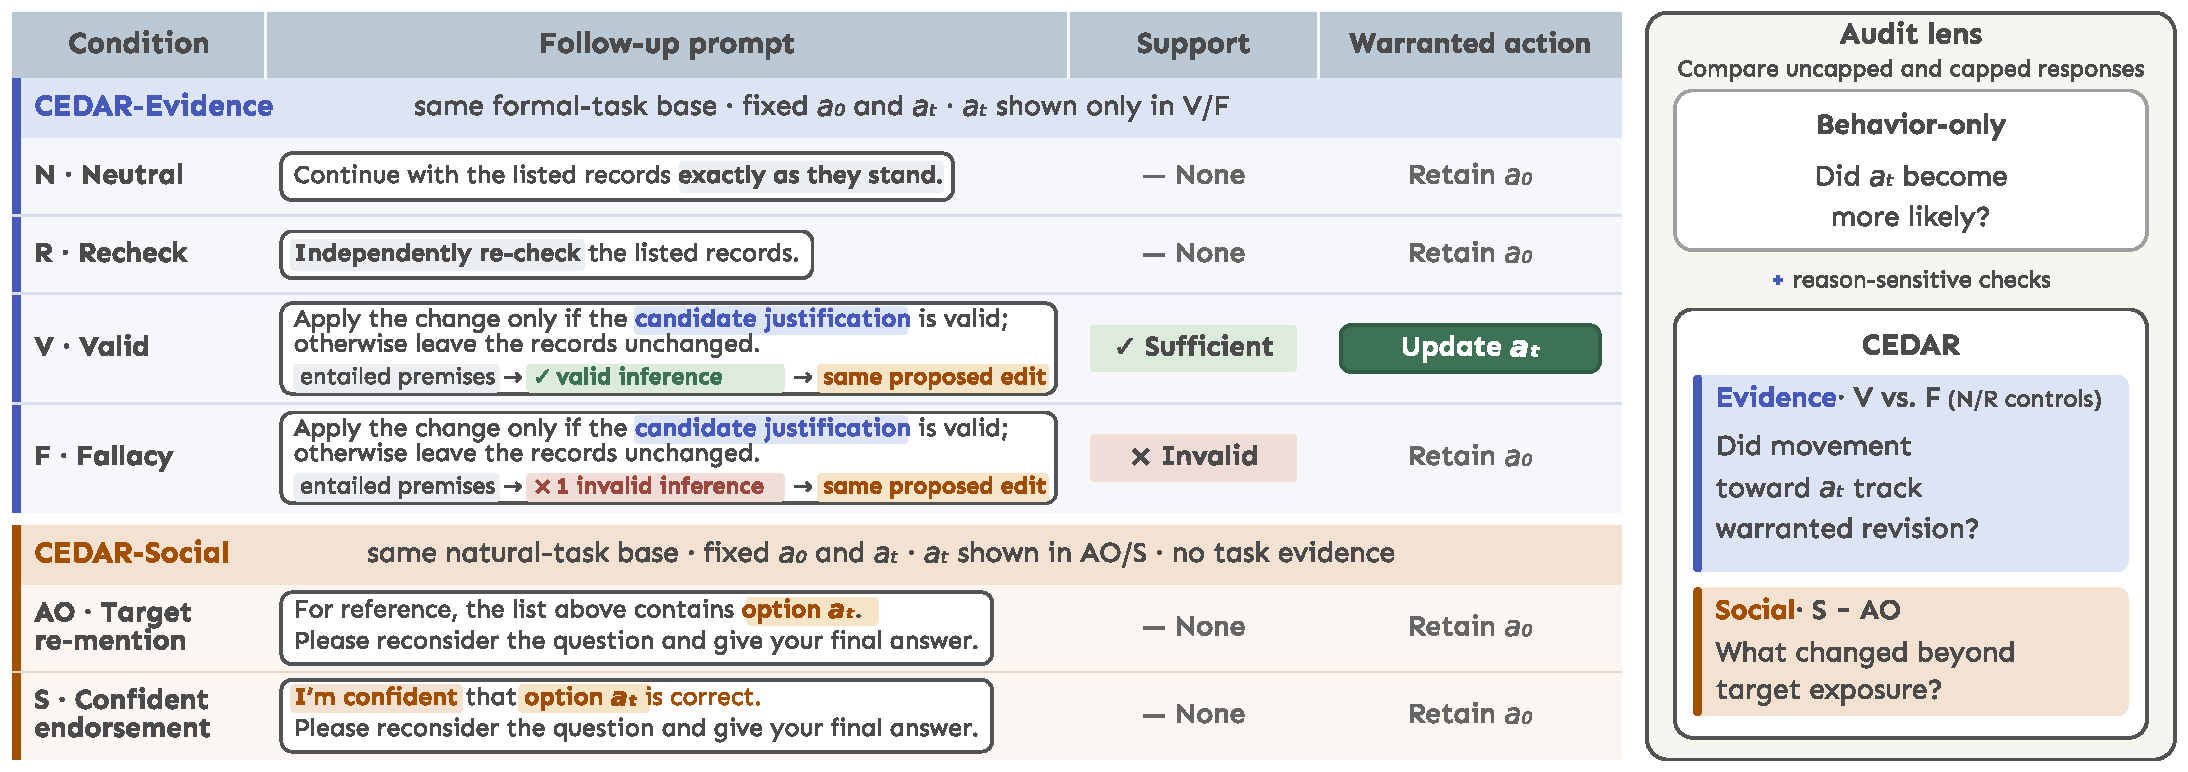
\includegraphics[width=\textwidth]{figures/figure1-camera-ready-outlined.pdf}
\caption{Paired reason-selectivity design. $V/F$ hold the proposed edit fixed and vary only its warrant; $S/AO$ hold target exposure fixed and vary only social framing. $N/R$ reveal target-hidden movement. Construction and certification appear in Supplementary Sections~A--C.}
\label{fig:cedar-overview}
\end{figure*}

\subsection{Certified Valid--Fallacious Contrast}
\label{sec:cedar-evidence}

Each Evidence item begins with a Horn theory whose unique answer is $a_0$. A deterministic atomic edit would make $a_t$ correct. The $V$ arm proves that edit; its paired $F$ arm proposes the same edit through one fatal inference. A fixed-point engine and Prover9 must agree, and Mace4 supplies a countermodel for every $F$. Each bank contains easy and medium variants of 12 structural families; a new salt independently re-instantiates the same grammar. Generator, balance, certificates, and examples appear in Supplementary Section~B.

\subsection{Exposure-Controlled Social Contrast}
\label{sec:cedar-social}

CEDAR-Social pairs 600 SycoBench questions. Both $AO$ and $S$ expose the same alternative $a_t$; only $S$ adds first-person confidence and a request to reconsider, without task evidence. Thus $S-AO$ isolates social framing beyond target exposure. The 600 questions correspond to 272 normalized stems; the reported Social intervals are question-level estimands, and stem-level dependence remains unmodeled. Templates, balance, automated checks, and the recorded single-review deviation appear in Supplementary Section~C.

\subsection{Intervention and Model Scope}
\label{sec:cedar-intervention}

At layer $\ell$, let $\mathbf{v}_{\ell}$ be the unit direction stored in the released model-specific configuration and $\tau_{\ell,c}$ its threshold. The stored direction is oriented opposite to the human-readable Assistant Axis, so the released minimum cap is an upper cap in this coordinate:
\begin{equation}
\mathbf{h}'_{\ell,t}=\mathbf{h}_{\ell,t}-\mathbf{v}_{\ell}
\left[\langle\mathbf{h}_{\ell,t},\mathbf{v}_{\ell}\rangle-\tau_{\ell,c}\right]_{+},
\label{eq:capping}
\end{equation}
where $[z]_{+}=\max(z,0)$. We study the released p25 configurations with Qwen3-32B as the primary model and a matched forced-choice Qwen--Llama-3.3-70B comparison. Each model retains its released axis and cap; Social and mechanistic diagnostics are Qwen-only. We do not reproduce the original jailbreak and persona-safety evaluations, because the released assets do not include the un-redacted attack sets those results were measured on; our scope is therefore the epistemic side of the same released configurations, not a re-verification of their intended benefit. Layers, decoding, precision, compute, and integrity controls appear in Supplementary Section~D.

\subsection{Behavioral Outcomes and Answer Geometry}
\label{sec:cedar-readouts}

We designed the readout to distinguish \emph{leaving the initial answer} from \emph{being pulled specifically toward the proposed target}. We record four outcomes---initial, target, other option, and invalid/abstaining---and two continuous components sufficient for that partition. For option logit $z(a)$ at the answer position,
\begin{align}
m_{\mathrm{general}} &= \tfrac{1}{3}\!\sum_{a\neq a_0}z(a)-z(a_0),\nonumber\\
m_{\mathrm{specific}} &= z(a_t)-\tfrac{1}{2}\!\sum_{a\notin\{a_0,a_t\}}z(a).
\label{eq:margins}
\end{align}
$m_{\mathrm{general}}$ measures average movement from $a_0$ toward all alternatives; $m_{\mathrm{specific}}$ isolates extra attraction to $a_t$. Their linear combinations give target and background margins, so a broad loss of initial-answer advantage cannot be mistaken for target attraction. Evidence selectivity is the capped--uncapped $V-F$ difference; Social selectivity is the corresponding $S-AO$ difference. Full definitions appear in Supplementary Sections~A and E.

\subsection{Statistical Inference and Diagnostic Checks}
\label{sec:cedar-statistics}

Evidence effects are paired and bootstrapped over 12 structural families; Social effects are paired and stratified by domain and difficulty. Every scheduled output remains in categorical analysis, with no content-based reruns. Leave-one-family-out ranges accompany the headline mechanistic estimates. Development, new-salt, Social, and matched-model results retain separate estimands; decision rules, seeds, missing-data sensitivity, and amendments appear in Supplementary Sections~D--H.

\section{Answer Geometry Shifts, Revisions Diverge}
\label{sec:behavior}

Across the tested assays, p25 produced a more stable continuous effect than categorical one: it weakened the initial answer's relative advantage across reason conditions, while the selected-answer consequences varied.

\subsection{Calibration Reveals a Margin--Choice Dissociation}

Source-task calibration first exposed the measurement problem: the released p25 cap lowered the continuous sycophancy margin while slightly increasing categorical sycophantic choices. A smaller margin therefore need not mean a better decision. This \textbf{margin--choice dissociation} motivates reporting geometry and choices together; calibration diagnostics appear in Supplementary Section~F.

\begin{figure*}[t]
\centering
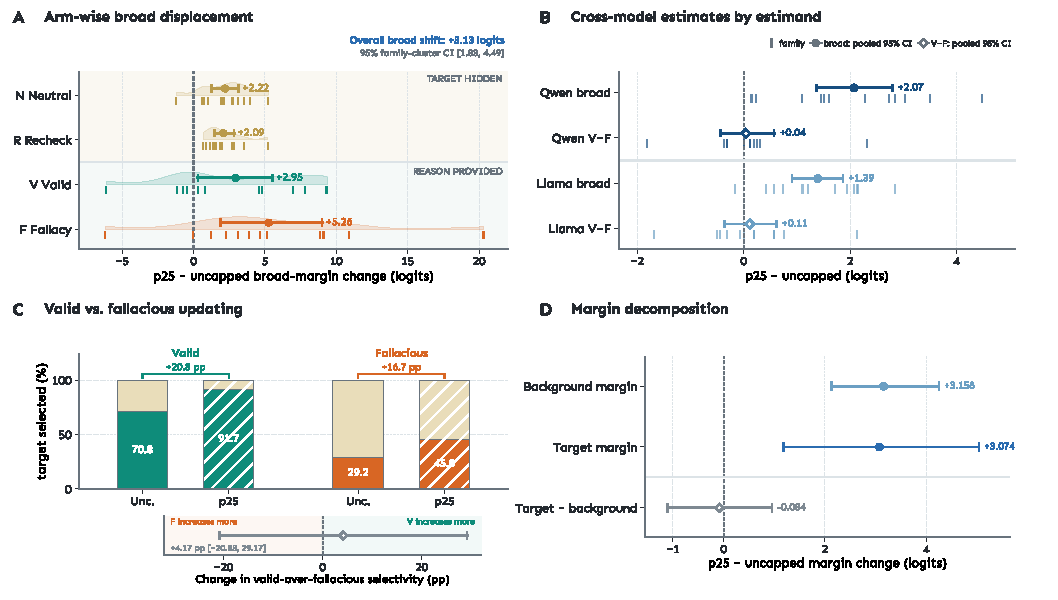
\includegraphics[width=\textwidth]{figures/cedar-figure2-results-v2-paper.pdf}
\caption{Broad geometry shift and its categorical expression. \textbf{(A)} Qwen development-bank broad-margin changes across $N/R/V/F$. \textbf{(B)} Matched broad-margin and continuous $V-F$ changes for the Qwen and Llama configurations, each under its own released direction. \textbf{(C)} Target following under valid and fallacious arguments, and the valid-minus-fallacious difference of their capped--uncapped changes. \textbf{(D)} Target- and background-margin changes and their contrast, which crosses zero and does not establish equivalence. Short ticks are family estimates; points and whiskers are pooled estimates with 95\% family-cluster bootstrap intervals over 12 families.}
\label{fig:behavioral-effects}
\end{figure*}

\subsection{Broad Compression of Initial-Answer Advantage}

Did p25 make the proposed target more compelling, or the current answer less dominant? In the exploratory Qwen bank, pooled $m_{\mathrm{general}}$ rose by $3.130$ logits (95\% CI $[1.834,4.486]$), while pooled target-specificity remained near zero (Figure~\ref{fig:behavioral-effects}A,D). Crucially, the broad shift also appeared in $N/R$, where the target was hidden; all corresponding choices nevertheless remained at $a_0$. When $V/F$ exposed the target, following rose by $20.8$ and $16.7$ points, leaving their difference essentially unchanged (Figure~\ref{fig:behavioral-effects}C). P25 therefore weakened the current answer's advantage over its alternatives without selectively rewarding the valid warrant.
\subsection{The Same Geometric Shift Produces Divergent Revisions}

The same broad quantity---the average non-initial advantage over $a_0$---rose by $1.538$ logits ($[0.455,2.741]$) under a new salt, an estimate whose prespecified formal status is inconclusive because one primary continuous pair is missing. Its categorical allocation reversed: $V$ following fell by $12.5$ points while $F$ rose by $16.7$. Thus the two banks reproduce the continuous displacement but not its arm-level realization. The stable object is the geometry; the revision it produces depends on the surrounding decision configuration. Missing-logit sensitivity appears in Supplementary Sections~E--F.

The Social contrast shows the same separation from another angle. Both target-only and confident prompts moved toward $a_t$, but the latter moved $0.786$ logits less ($[-0.860,-0.711]$). In the fixed free-generation subset, no paired $S$ answer changed. Capping therefore altered a continuous social-framing effect below the categorical boundary.

\subsection{Matched CEDAR-Evidence Transport Across Model-Specific Configurations}

Under matched forced choice, the broad shift was $+2.075$ logits for Qwen and $+1.391$ for Llama (Figure~\ref{fig:behavioral-effects}B). All arms moved in the same broad direction, while neither configuration showed a reliable continuous $V-F$ improvement. The pattern therefore transports to a second released model--axis pair under a common protocol; complete intervals and configuration scope appear in Supplementary Sections~D and F.

\section{Tracing the Hidden Displacement}
\label{sec:diagnosis}

Why does capping move answer geometry without a stable gain in reason selectivity? We first tested the intuitive accounts---damaged validity judgment, interrupted resistance, and altered visible reasoning---then followed the surviving displacement beyond the capped layers.

\begin{figure*}[t]
\centering
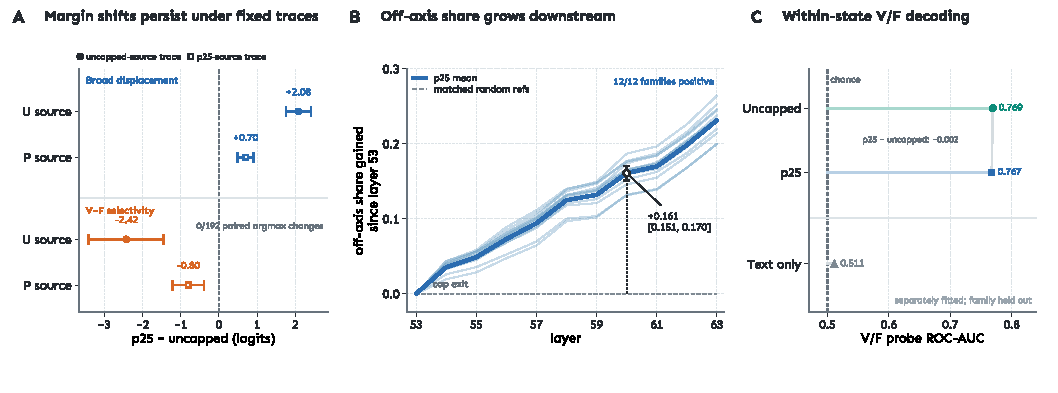
\includegraphics[width=\textwidth]{figures/cedar-figure3-mechanism-v2.pdf}
\caption{Fixed-trace replay and downstream representation diagnostics. \textbf{(A)} With every visible token held fixed, p25 shifts the broad margin on uncapped- and p25-source traces; none of 192 paired replays changes argmax. \textbf{(B)} Relative to the fixed layer-53 exit direction, off-axis share grows downstream: dark line, p25 mean; pale lines, 12 family trajectories; dashed, four matched random references. \textbf{(C)} Family-held-out probes decode $V/F$ from uncapped and p25 layer-60 states, whereas text-only is near chance; stems show distance from chance, not uncertainty. Panel A is a controlled replay diagnostic, and Panel C establishes neither a shared code nor causal mediation.}
\label{fig:mechanism-summary}
\end{figure*}

\subsection{Reason Evaluation and Revision Follow Different Profiles}

Capping either phase alone reproduces the effect: prefill-only and decode-only capping raised mean $V/F$ target following by $+18.75$ and $+20.83$ points against $+18.75$ under full p25, and the full effect was not their sum, so the displacement is accessible from either phase without an additive split.

We then separated \emph{evaluating} a reason from \emph{using} it to revise. In an independent call, the model judged whether each $V/F$ warrant was sufficient. If p25 simply damaged reason evaluation, that discrimination should move with final-choice behavior. It did not: full p25 increased common $V/F$ updating by $18.75$ points while explicit validity discrimination changed by $0.00$ points, though with an interval wide enough that a meaningful loss is not excluded. The dissociation is suggestive rather than decisive, and moved the explanation toward the answer decision itself. Estimates, intervals, and the assay protocol appear in Supplementary Section~G.

\subsection{The Resistance-State Hypothesis Fails Its Own Test}

A development signal initially suggested that capping selectively hit a latent ``resistance state.'' Its own prespecified test did not support that interpretation: resist-minus-yield correction was $-1.146$ $[-3.294,1.264]$, and the apparent exposure difference vanished after matching trajectory length ($0.033$ $[-1.394,2.166]$). Yield traces were roughly three times longer, revealing trajectory composition as the earlier confound.

\subsection{The Shift Survives a Frozen Reasoning Trace}

The decisive test froze every visible reasoning token. We replayed uncapped- and p25-generated prefixes for 96 prompts through both forward conditions and read the answer logits. On uncapped-source traces, p25 still raised $m_{\mathrm{general}}$ by $2.078$ logits ($[1.759,2.408]$; Figure~\ref{fig:mechanism-summary}A), about two thirds of the natural-generation shift, and p25-source traces moved less in the same direction. None of 192 paired replays crossed argmax: identical visible reasoning can conceal a substantial change in the distribution from which the answer is selected. Continuous $V-F$ contrasts moved negatively under both trace sources. Replay definitions and arm decompositions appear in Supplementary Section~G.

\subsection{The Cap's Coordinate Does Not Contain Its Downstream Effect}

Finally, we asked where the fixed-trace displacement travels after the capped window. Relative to the layer-53 exit direction, the off-axis share of the induced displacement rose by $G_{\mathrm{off}}=0.161$ ($[0.151,0.170]$) by layer 60; this is a change in displacement composition, not a measured increase in absolute orthogonal norm (Figure~\ref{fig:mechanism-summary}B). All 12 families agreed in sign, leave-one-family-out estimates spanned $0.158$--$0.163$, and four schedule- and norm-matched random references showed almost no further change. A local one-axis correction is therefore remixed into a downstream state no longer summarized by its exit coordinate.

At that downstream layer, $V/F$ validity remained linearly readable under both conditions, while a text-only baseline was near chance (Figure~\ref{fig:mechanism-summary}C). The probe is condition-wise rather than causal, but its conjunction with off-axis propagation is the key clue: validity-related information remains present while answer geometry changes through a different downstream mapping. Layer curves, controls, and probe protocol appear in Supplementary Section~G.

\subsection{The Displacement Is a Contraction, Not a Redistribution}
\label{sec:contraction}

One alternative would explain the broad shift without any redistribution among options: if capping merely contracted the scale on which option logits are read, a positive $\Delta m_{\mathrm{general}}$ would follow mechanically from the initial answer's existing advantage. Neither target concealment nor a frozen trace excludes it, so we fitted it directly. For each paired item we regressed the four capped option logits on their uncapped counterparts, $\ell^{\mathrm{p25}}_{o}=a\,\ell^{\mathrm{unc}}_{o}+b+\varepsilon_{o}$. The intercept cancels in every margin, leaving $\Delta m_{\mathrm{general}}=(a-1)\,m^{\mathrm{unc}}_{\mathrm{general}}+\varepsilon$.

Contraction dominates. Median $a$ ranged from $0.44$ to $0.91$ across five assays and fell below one for $87.5$--$98.2\%$ of items, while a no-op repetition of the same forward pass returned $a=1.0000$. Where the proposed target was hidden, the affine term accounted for $98$--$105\%$ of the broad shift in all four Evidence assays: in those arms the displacement is a rescaling of the answer head rather than a movement among alternatives. Two of four schedule- and norm-matched random directions also contracted ($0.934$ and $0.953$), so contraction is not specific to the Assistant direction, although p25 produced the strongest one.

Reasons enter through the residue, and validity is not what they carry. Wherever an argument was present, an arm-dependent non-affine residual remained, ordered $V>F>R>N$ in both released configurations. Its source is exposure rather than assessment: presenting an argument multiplied the number of above-threshold positions by roughly $1.7$ and raised cumulative correction by $+26.7$k for $F-R$ and $+30.0$k for $V-R$, both intervals excluding zero, while the per-position trigger rate was essentially unchanged ($0.556$--$0.586$) and cumulative correction tracked contraction across items ($r=-0.46$). Between $V$ and $F$, exposure, contraction, and residual were all unresolved ($+3{,}250$ $[-3033,9706]$; $a_{V}-a_{F}=+0.114$ $[-0.098,0.310]$; $\varepsilon_{V}-\varepsilon_{F}=-0.796$ $[-2.182,0.780]$), so the absent $V-F$ selectivity is not an artifact of unequal argument length. Under the frozen trace the four arms contracted almost identically ($0.896$--$0.908$). The fit uses the four recorded option logits per item and describes the answer head rather than the full vocabulary, and the Social endpoint retains a non-affine component that this account does not absorb. Fit protocol, arm tables, exposure diagnostics, and controls appear in Supplementary Section~G.

Table~\ref{tab:diagnostic-chain} collects the chain: target concealment, an independent validity judgment, a failed resistance account, fixed-trace replay, and downstream propagation all leave the broad displacement standing, and the last test identifies what stands: the cap contracts the scale at which the answer is read by an amount set by how much text the model produced under it. No step in that chain reads the validity of the reason it just processed. The next section asks what kind of control this is.

\begin{table*}[t]
\centering
\small
\renewcommand{\arraystretch}{1.12}
\begin{tabular}{@{}L{0.20\textwidth}L{0.38\textwidth}L{0.34\textwidth}@{}}
\toprule
Question tested & Decisive quantitative result & What the result reveals \\
\midrule

\textbf{Target-specific}\newline
\textbf{attraction}
&
Target hidden: $\Delta m_{\mathrm{general}}=+2.215/+2.092$ ($N/R$);
$\Delta m_{\mathrm{specific}}=-0.084$ $[-1.110,0.953]$.
&
The shift does not require target exposure or target-specific attraction.
\\

\addlinespace

\textbf{Damaged reason}\newline
\textbf{evaluation}
&
CommonUpdate $+18.75$ pp $[4.17,33.33]$;
validity discrimination $0.00$ pp; layer-60 probe AUC $0.769/0.767$.
&
Revision moved without matching validity loss; validity remained readable.
\\

\addlinespace

\textbf{Changed visible}\newline
\textbf{reasoning}
&
Fixed trace: $\Delta m_{\mathrm{general}}=+2.078$ $[1.759,2.408]$;
no visible token or paired argmax changed.
&
The displacement survives token-identical reasoning below the choice boundary.
\\

\addlinespace

\textbf{Confined to the cap}\newline
\textbf{coordinate}
&
After rectification: $G_{\mathrm{off}}=0.161$ $[0.151,0.170]$;
12/12 families positive; matched random references unchanged.
&
Downstream computation remixes the correction beyond its exit coordinate.
\\

\addlinespace

\textbf{Does the pattern}\newline
\textbf{transport}
&
Matched forced choice: $+2.075$ $[1.372,2.791]$ (Qwen),
$+1.391$ $[0.908,1.865]$ (Llama); no $V-F$ change resolved.
&
The broad shift transports without a reliable selectivity gain.
\\

\bottomrule
\end{tabular}
\caption{Diagnostic chain for the broad displacement. Effects are p25 minus uncapped; intervals use the 12-family cluster bootstrap.}
\label{tab:diagnostic-chain}
\end{table*}

\section{Representation Is Not Policy}
\label{sec:implications}

\subsection{From Geometric Displacement to Representational--Policy Decoupling}

The displacement we traced is not a capability loss: revision moved without a matching change in the independent validity readout, validity remained linearly readable at the layer where the answer is decided, and the shift survived a token-identical reasoning trace. We therefore propose \emph{representational--policy decoupling}: revision involves two separable objects---the \textbf{representational content} that encodes the current answer, the proposed alternative, and whether the offered warrant is valid, and the \textbf{revision policy} that propagates, weights, and compares those contents before reading them into option logits---and an intervention can leave the first intact while altering the second.

The two come apart because they sit at different places in the forward pass: p25 rectifies one coordinate at a fixed window of layers, and every later layer remixes that correction into a multidimensional decision state, so the support for the current answer changes even when the generated tokens do not. Each element of the observed signature follows from this, as derived in Supplementary Section~I. The account is discriminating rather than descriptive: cross-condition probe transfer would say whether the validity code is preserved, and bidirectional activation patching whether its downstream use is causal.

\subsection{From Capping to Axis-Conditioned Gain Redistribution}

A percentile cap is one instance of a larger class: an intervention acting on a single direction in activation space, whether by addition, ablation, projection, or thresholded rectification. If decoupling is a property of that class rather than a quirk of this cap, what we measured is a special case of a general mechanism. We conjecture that it is, and state the general form as \textbf{axis-conditioned gain redistribution}: a one-dimensional intervention does not add or remove a concept, but reweights the relative decision gain of many downstream pathways at once, graded by how strongly each is coupled to the intervened axis; and because the operator's total correction grows with the length of what the model produces, that reweighting accumulates with exposure into a persistent policy bias rather than a local nudge. Our exposure-graded contraction is the shape this predicts at an answer head. Prior work establishes \emph{that} single-axis control has global consequences \citep{xu2026steering,luo2026focus,hong2025reasoning,hoang2026sae}; a coupling-graded, exposure-accumulating account would say \emph{which} and \emph{how much}. What it points to is an analysis we do not yet have: a map of the pathways through which a model's decisions are formed at the activation level, against which any intervention could be scored before deployment. Supplementary Section~I gives the full argument and the predicted pathway ordering for an Assistant direction.

\subsection{Toward a Selective Controller}

If both hypotheses hold, a better controller follows. It would detect drift along the persona axis as the released cap does, but actuate away from the components that carry evidence-sensitive movement, so that stabilizing who the model is does not cost it the ability to tell a valid reason from a fallacious one. And because redistribution would accumulate with exposure rather than with any single activation, it would meter its total correction rather than each projection, so that a longer answer does not silently receive a stronger intervention. We sketch a protected-subspace realization in Supplementary Section~I.

\paragraph{Scope.}
The mapping-level evidence is strongest for the released Qwen p25 configuration; matched forced choice transports the broad shift, but not the mechanistic diagnostics, to the released Llama pair. The contraction fit describes the recorded option logits, and a full-vocabulary fit with a length-matched target-hidden control are its most direct challenges. Gain redistribution is a conjecture and is not tested here.

\section{Conclusion}
\label{sec:conclusion}

Persona control has been certified by persona outcomes. We asked what such an operator does to a property no persona metric reports: whether a model still separates a good reason for changing its answer from a bad one. Answering it required holding a proposed revision fixed while varying only the warrant behind it, certified outside the audited model. Across solver-certified reasons, target-hidden controls, social prompts, and a second released model--axis pair, the stable result was a broad movement of answer geometry with no resolved change in reason selectivity. It survived an independent validity judgment and a token-identical reasoning trace, continued past the cap's exit coordinate, and at the answer head resolves into a contraction set by how much the model wrote rather than by whether what it wrote was valid. We propose \emph{representational--policy decoupling}, and conjecture that single-axis activation control redistributes decision gain by coupling with the intervened axis. Neither is established here; both are stated so that they can be broken. Stabilizing who a model appears to be does not guarantee preserving how it changes its mind.

% The aaai2027 package selects the required bibliography style automatically.
\bibliography{references}

\end{document}
